\documentclass{llncs}
\pagestyle{plain}
\usepackage[show]{ed}
\usepackage[utf8]{inputenc}
\usepackage{lststex}
\usepackage{paralist}
\lstset{basicstyle=\sf,columns=fullflexible,showstringspaces=false}
% \usepackage{url}
% \usepackage{wrapfig}
\usepackage{tikz,standalone}
\usetikzlibrary{backgrounds,shapes,fit,shadows}
\makeatletter%%%%%%%%%%%%%%%%%%%%%%%%%%%%%%%%%%%%%%%%%%%%%%%%%%%%%%%%%%%%%%%%%
% A TIKZ library for MMT Theory Graphs
% copyright 2014 Michael Kohlhase; Released under the LPPL
%%%%%%%%%%%%%%%%%%%%%%%%%%%%%%%%%%%%%%%%%%%%%%%%%%%%%%%%%%%%%%%%%
%
% this library provides some standardized node and arrow styles for formatting MMT graph
% diagrams in tikz. The advantage is that we can classify the arrows and nodes
% symbolically and with the styles in this library achieve a uniform look that helps
% readability. 
%
%%%%%%%%%%%%%%%%%%%%%%%%%%%%%%%%%%%%%%%%%%%%%%%%%%%%%%%%%%%%%%%%%

%%% 1. Theories
% a generic theory
\def\outerthysep{.3mm}
\def\innerthysep{.5mm}
\tikzstyle{thy}=[draw,outer sep=\outerthysep,rounded corners,inner sep=\innerthysep]
% a primitive theory
\tikzstyle{primthy}=[thy,double]
% a theory graph 
\tikzstyle{thygraph}=[draw,outer sep=1mm,rounded corners,dashed]

%%% 2. Arrows 
%%% 2.1. Arrowtips (only internal)
\usetikzlibrary{arrows}
\newcommand{\@mmtarrowtip}{angle 45}
\newcommand{\@mmtreversearrowtip}{angle 45 reversed}
\newcommand{\@mmtarrowtipepi}{triangle 45}
\newcommand{\@mmtarrowtipmonoright}{right hook}
\newcommand{\@mmtarrowtipmonoleft}{left hook}
\newcommand{\@mmtarrowtippartial}{right to}
\newcommand{\@mmtarrowtippartialleft}{left to}
\newcommand{\@mmtreversearrowtippartial}{right to reversed}
\newcommand{\@mmtreversearrowtippartialleft}{left to reversed}

%%% 2.2 the arrow sstyles in graphs
\usetikzlibrary{decorations,decorations.pathmorphing,decorations.markings}
% any morphism 
\tikzstyle{morph}=[-\@mmtarrowtip,thick] 
\tikzstyle{mapsto}=[|-\@mmtarrowtip] %| any morphism 
% structures
\tikzstyle{struct}=[-\@mmtarrowtip,thick]
% inclusions: regular, partial, and left variants
\tikzstyle{include}=[\@mmtarrowtipmonoright-\@mmtarrowtip,thick]
\tikzstyle{revinclude}=[\@mmtarrowtip-\@mmtarrowtipmonoright,thick]
\tikzstyle{pinclude}=[\@mmtarrowtipmonoright-\@mmtarrowtippartial,thick]
\tikzstyle{includeleft}=[\@mmtarrowtipmonoleft-\@mmtarrowtip,thick]
\tikzstyle{pincludeleft}=[\@mmtarrowtipmonoleft-\@mmtarrowtippartialleft,thick]
% views: regular, mono, partial, and left variants
\tikzstyle{preview}=[decorate,
                                decoration={coil,aspect=0,amplitude=1pt,
                                                    segment length=6pt,
                                                    pre=lineto,pre length=3pt,
                                                    post=lineto,post length=5pt},
                                thick]
\tikzstyle{view}=[preview,-\@mmtarrowtip]
\tikzstyle{mview}=[preview,\@mmtarrowtipmonoright-\@mmtarrowtip]
\tikzstyle{pview}=[preview,-\@mmtarrowtippartial]
\tikzstyle{pmview}=[preview,\@mmtarrowtipmonoright-\@mmtarrowtippartial]
\tikzstyle{viewleft}=[preview,-\@mmtarrowtip]
\tikzstyle{mviewleft}=[preview,\@mmtarrowtipmonoleft-\@mmtarrowtip]
\tikzstyle{pviewleft}=[preview,-\@mmtarrowtippartialleft]
\tikzstyle{pmviewleft}=[preview,\@mmtarrowtipmonoleft-\@mmtarrowtippartialleft]
\tikzstyle{adoption}=[preview,thin,double,-\@mmtarrowtip]
% biviews: regular, partial, and left variants
\tikzstyle{biview}=[preview,\@mmtarrowtip-\@mmtarrowtip]
\tikzstyle{pbiview}=[preview,\@mmtreversearrowtippartial-\@mmtarrowtippartial]
\tikzstyle{pbiviewleft}=[preview,\@mmtreversearrowtippartialleft-\@mmtarrowtippartialleft]
% defining views (experimental)
\tikzstyle{defview}=[preview,densely dotted,-\@mmtarrowtip]
% meta-theory inclusion
\tikzstyle{meta}=[dotted,-\@mmtarrowtip,thick]
% conservative extensions (abbreviation)
\tikzstyle{conservative}=[hooks-\@mmtarrowtip,double] 
% conservative development
\tikzstyle{conservdev}=[hooks-\@mmtarrowtip,dashed,double] 

% antimorphisms as striktthroughs
\tikzset{anti/.style={
    decoration={markings, mark=between positions 0.2 and 0.8 step 4mm with {
        \draw [thick,-] ++ (-3pt,-3pt) -- (3pt,3pt);}},
    postaction={decorate}}}

% parallel markup
\tikzstyle{parallel}=[\@mmtarrowtip-\@mmtarrowtip,dashed]

%%%% 3. Realms 
\tikzstyle{prerealm}=[draw=blue!40,rectangle,rounded corners,inner sep=10pt,inner ysep=20pt]
\tikzstyle{realm}=[prerealm,fill=gray!4]
\tikzstyle{pillar}=[prerealm,fill=gray!10]

%%% 4. convenience macros
%%% 4.1 the \mmtthy macro takes three arguments, name, decl, axioms and makes a 
% table-like structure
\newcommand\mmtthy[3]{\def\@second{#2}\def\@third{#3}%
\begin{array}{l}\textsf{#1}%
\ifx\@second\@empty\else\\\hline #2\fi%
\ifx\@third\@empty\else\\\hline #3\fi%
\end{array}}
%%% 4.2 the \mmtar takes two arguments, some tikz options, and an arrow style. \nmmtar
% is a variant that also has a name on top.
\newcommand\mmtar[2][]{\raisebox{.5ex}{\tikz[#1]{\draw[#2] (0,0) -- (.6,0);}}}
\newcommand\nmmtar[3][]{\raisebox{.4ex}{\tikz[#1]{\draw[#2] (0,0) --
      node[above]{\ensuremath{\scriptstyle #3}} (.8,0);}}}
%%%% 3.3 Pushout symbols
%%  (after http://tex.stackexchange.com/questions/1144/pushouts-and-pullbacks)
%% \nepushout[<pos>]{<basenode>}{<targetnode>} positions a pushout symbol 
%% (available separately as \pushoutsymb) <pos> of the way between <basenode>
%%  and <targetnode>. 
\usetikzlibrary{calc}
\newcommand\@pushout[4][]{\def\@test{#1}%
\ifx\@test\@empty\def\@@num{.5}\else\def\@@num{#1}\fi%
\begin{scope}[shift=($(#2)!\@@num!(#3)$)]\@nameuse{@#4pushoutsymb}\end{scope}} 
\newcommand\@nepushoutsymb{\draw +(-.2,0) -- +(0,0)  -- +(0,-.2);\fill +(-.1,-.1) circle (.03);}
\newcommand\nepushoutsymb{\tikz{\@nepushoutsymb}}
\newcommand\nepushout[3][]{\@pushout[#1]{#2}{#3}{ne}}

\newcommand\@sepushoutsymb{\draw +(-.2,0) -- +(0,0)  -- +(0,.2);\fill +(-.1,.1) circle (.03);}
\newcommand\sepushoutsymb{\tikz{\@sepushoutsymb}}
\newcommand\sepushout[3][]{\@pushout[#1]{#2}{#3}{se}}

\newcommand\@nwpushoutsymb{\draw +(.2,0) -- +(0,0)  -- +(0,-.2);\fill +(.1,-.1) circle (.03);}
\newcommand\nwpushoutsymb{\tikz{\@nwpushoutsymb}}
\newcommand\nwpushout[3][]{\@pushout[#1]{#2}{#3}{nw}}

\newcommand\@swpushoutsymb{\draw +(.2,0) -- +(0,0)  -- +(0,.2);\fill +(.1,.1) circle (.03);}
\newcommand\swpushoutsymb{\tikz{\@swpushoutsymb}}
\newcommand\swpushout[3][]{\@pushout[#1]{#2}{#3}{sw}}

\newcommand\@npushoutsymb{\draw +(-.1,-.1) -- +(0,0)  -- +(.1,-.1);\fill +(0,-.1) circle (.03);}
\newcommand\npushoutsymb{\tikz{\@npushoutsymb}}
\newcommand\npushout[3][]{\@pushout[#1]{#2}{#3}{n}}

\newcommand\@spushoutsymb{\draw +(-.1,.1) -- +(0,0)  -- +(.1,.1);\fill +(0,.1) circle (.03);}
\newcommand\spushoutsymb{\tikz{\@spushoutsymb}}
\newcommand\spushout[3][]{\@pushout[#1]{#2}{#3}{s}}

\newcommand\@wpushoutsymb{\draw +(-.1,-.1) -- +(0,0)  -- +(-.1,.1);\fill +(-.1,0) circle (.03);}
\newcommand\wpushoutsymb{\tikz{\@wpushoutsymb}}
\newcommand\wpushout[3][]{\@pushout[#1]{#2}{#3}{w}}

\newcommand\@epushoutsymb{\draw +(.1,.1) -- +(0,0)  -- +(.1,-.1);\fill +(.1,0) circle (.03);}
\newcommand\epushoutsymb{\tikz{\@epushoutsymb}}
\newcommand\epushout[3][]{\@pushout[#1]{#2}{#3}{e}}

%%%%%% testing them: 
% \begin{tikzpicture}[scale=1.5]
%   \node (a) at (0,0) {a};
%   \node (b) at (1,0) {b};
%   \node (c) at (1,1) {c};
%   \node (d) at (0,1) {d};
%   \nepushout[.8]{a}c;
%   \nwpushout[.8]{b}d;
%   \sepushout[.8]{d}b;
%   \swpushout[.8]{c}a;
%   \draw (a) -- (b) -- (c) -- (d) -- (a);
%   \node (aa) at (4,0) {a};
%   \node (bb) at (3.5,.5) {b};
%   \node (cc) at (4,1) {c};
%   \node (dd) at (4.5,.5) {d};
%   \draw (aa) -- (bb) -- (cc) -- (dd) -- (aa);
%   \npushout[.8]{aa}{cc};
%   \spushout[.8]{cc}{aa};
%   \wpushout[.8]{bb}{dd};
%   \epushout[.8]{dd}{bb};
% \end{tikzpicture}

%%% Local Variables:
%%% mode: latex
%%% TeX-master: "test"
%%% End:
\makeatother
\usepackage{wrapfig}
\usepackage{xspace}
\usepackage{hyperref}
\usepackage{stex-logo}
\usepackage{odksystems}
\usepackage[style=alphabetic,backend=bibtex,isbn=false]{biblatex}
\addbibresource{kwarc.bib}% do not change
\addbibresource{rest.bib}% add bibs here!
\renewbibmacro*{event+venue+date}{}
\renewbibmacro*{doi+eprint+url}{%
  \iftoggle{bbx:doi}
    {\printfield{doi}\iffieldundef{doi}{}{\clearfield{url}}}
    {}%
  \newunit\newblock
  \iftoggle{bbx:eprint}
    {\usebibmacro{eprint}}
    {}%
  \newunit\newblock
  \iftoggle{bbx:url}
    {\usebibmacro{url+urldate}}
    {}}
% temporary fix due to http://tex.stackexchange.com/questions/311426/bibliography-error-use-of-blxbblverbaddi-doesnt-match-its-definition-ve
\makeatletter\def\blx@maxline{77}\makeatother

\title{Interoperability in the \ODK Project:\\
The Math-in-the-Middle Approach}

\author{
Paul-Olivier Dehaye\inst{1} 
Mihnea Iancu\inst{2} 
Michael Kohlhase\inst{2} 
Alexander Konovalov\inst{3} 
Samuel Lelièvre\inst{4} 
Dennis M\"uller\inst{2} 
Markus Pfeiffer\inst{3} 
Florian Rabe\inst{2} 
Nicolas~M.~Thiéry\inst{4} 
Tom Wiesing\inst{2}}

\institute{
  University of Z\"urich \and 
  Jacobs University \and 
  University of St~Andrews \and
  Universit\'e Paris-Sud
}
\providecommand\ifprefchar[2]{}% fix biblatex
\newcommand\defemph[1]{\textbf{#1}}

\begin{document}
\maketitle
\begin{abstract}
  \ODK\, -- ``Open Digital Research Environment Toolkit for the Advancement of
  Mathematics'' -- is an H2020 EU Research Infrastructure project that aims at supporting,
  over the period 2015--2019, the ecosystem of open-source mathematical software
  systems. \ODK will deliver a flexible toolkit enabling research groups to set
  up Virtual Research Environments, customised to meet the varied needs of research
  projects in pure mathematics and applications.

  An important step in the \ODK endeavor is to foster the interoperability between a
  variety of systems, ranging from computer algebra systems over mathematical databases to
  front-ends. This is the mission of the integration work package. We report on
  experiments and future plans with the \emph{Math-in-the-Middle} approach. This
  architecture consists of a central mathematical ontology that documents the domain and
  fixes a joint vocabulary, or even a language, going beyond existing systems such as
  OpenMath, combined with specifications of the functionalities of the various
  systems. Interaction between systems can then be enriched by pivoting around this
  architecture.
\end{abstract}

\section{Introduction}\label{sec:intro}

\begin{newpart}{MK: adapted from Tom's Thesis}
There is a large and vibrant ecosystem of open-source mathematical software systems.
These systems can range from calculators, which are only capable of performing simple
computations, via mathematical databases (curating collections of a mathematical objects)
to powerful modeling tools and computer algebra systems (CAS). 

Most of these systems are very specific -- they focus on one or very few aspects of
mathematics.  For example, the ``Online Encyclopedia of Integer Sequences''
(OEIS~\cite{Sloane:oeis12,oeis}) focuses on sequences over $\mathbb{Z}$ an their
properties and the ``L-Functions and Modular Forms Database''
(LMFDB)~\cite{Cremona:LMFDB16,lmfdb:on} objects in number theory pertaining to Langland's
program.  GAP~\cite{GAP:on} excels at discrete algebra, whereas
SageMath~\cite{SageMath:on} focuses on Algebra and Geometry in general, and
Singular~\cite{singular:on} on polynomial computations, with special emphasis on
commutative and non-commutative algebra, algebraic geometry, and singularity theory.

For a mathematician however (a user; let us call her Jane) the systems themselves are not relevant, instead she only cares about being able to solve problems. 
Typically, it is not possible to solve a mathematical problem using only a single program. 
Thus Jane needs to work with multiple systems and combine the results to reach a solution. 
Currently there is very little help with this practice, so Jane has to isolate sub-problems the respective systems are amenable to, formulate them into the respective input language, collect results, and reformulate them for the next system a tedious and error-prone process at best, a significant impediment to scientific progress in its overall effect. 
Solutions for some situations certainly exist, which can help get Jane unstuck, but these are ad-hoc and for specific, often-used system combinations only. 
Each of these requires a lot of maintenance and does not scale to a larger set of specialist systems. 

The OpenDreamKit project, which aims at a mathematical VRE toolkit, proposes the Math-in-the-Middle (MitM~\cite{DehKohKon:iop16}) Paradigm, an interoperability framework based on a flexiformal
representation of mathematical knowledge and aligns this with system-generated interface
theories. 

In this paper we instantiate the MitM paradigm with a concrete domain development and
evaluate it on a distributed computing GAP, SageMath and Singular.\ednote{ we generally we
  want to show that the promises in the CICM paper become reality.}

We will use the following example as a running example: Jane wants to act on singular
polynomials with GAP permutation groups\ednote{MK@(MP|VA): }

 \ednote{MK: continue with the structure} 
\end{newpart}

%%% Local Variables:
%%% mode: latex
%%% TeX-master: "paper"
%%% End:

\section{The \ODK project (2015-2019)}\label{sec:odk}

The \ODK project runs for four years, starting in September 2015, and
involves about 50 people spread over 15 sites in Europe, with a total
budget of 7.6 million euros. The largest portion of that is devoted to
employing an average of 11 researchers and developers working full
time on the project, while the other participants contribute the
equivalent of six people working full time.

\ODK's goal is to develop \emph{Virtual Research Environments}
(VRE), that is online services enabling groups of researchers,
typically spread across many countries, to work collaboratively on a per project
basis. Rather than constructing a large monolithic VRE, we have
designed our proposal around the long-term investments listed in the
previous section, working on the large scale yet modular integration
of mathematical software. Our goal is a modular, interoperable,
and customisable VRE toolkit built out of relatively modest
components, interfaced through our approach to work on the grease to
make this work.
According to the funding scheme, the project addresses, besides
its technical goals, aspects such as outreach, dissemination, or tools
to support teaching.

% \ednote{NT: The following paragraph is a political message; not sure
%   it fits there; in case we need to save a bit of space, that's one of
%   the first things to cut out}
An innovative aspect of the \ODK project is that its preparation and management happens,
as much as is practical and without infringing on privacy, in the open. For example, most
documents, including the proposal itself, are version controlled on public repositories
and progress on tasks and deliverables is tracked using public issues
(see~\cite{OpenDreamKit:on}). This has proven a strong feature to collaborate tightly with
the community and get early feedback.

In practice, \ODK's work plan consists of several work packages: component architecture
(modularity, packaging, distribution, deployment), user interfaces (\Jupyter interactive
notebook interfaces, 3D visualization, documentation tools), high performance mathematical
computing (especially on multicore/parallel architectures), a study of social aspects of
collaborative software development, and a package on data/knowledge/software-bases.

The latter package focuses on the identification and extension of ontologies and standards
to facilitate safe and efficient storage, reuse, interoperation and sharing of rich mathematical
data, whilst taking provenance and citability into account.
Its outcome will be a component architecture for semantically sound data archival and sharing,
and integrate computational software and databases. The aim is to enable researchers to seamlessly
manipulate mathematical objects across computational engines (e.g. switch algorithm implementations
from one computer algebra system to another), front end interaction modes (database queries, notebooks,
web, etc) and even backends (e.g. distributed vs.~local).

In this paper, we discuss the general approach chosen to develop this semantically aware component
architecture. 

% The \ODK project is committed to working openly. Deliverables are tracked using public GitHub issues (see~\cite{OpenDreamKit:on}), which tightens the loop for early community feedback.

%%% Local Variables:
%%% mode: latex
%%% TeX-master: "paper"
%%% End:

%  LocalWords:  specialized Arxiv Jupyter IPython ldots compactitem emph compactenum odk
%  LocalWords:  ODKproposal organization standardization visualization citability oldpart
%  LocalWords:  organizing Swinnerton-Dyer resentation desingularisation Hironaka ednote
%  LocalWords:  Hironaka algorithmisation Villamayor

The \pn project intends to integrate multiple mathematical software systems into a VRE
toolkit. These systems are constituted by large collections of algorithms manipulating
highly optimized data structures representing mathematical objects with the intent of
solving specific computational problems. The systems overlap in the mathematical
objects they cover and the problems they can solve, but every system has aspects that are
not covered by any other system (as efficiently or generally). In particular, algorithms,
implementation languages, and data structures differ significantly between systems and are
optimized to their particular domain and intended performance profile. As the systems
represent decades worth of experience and development, a re-implementation is prohibitive
in cost and might lead to systems with greater coverage, but less efficiency.

Given this situation, the integration problem in \pn becomes a problem of establishing an
interoperability layer between systems. As we have seen in the previous section, the
mathematical knowledge -- for specifying the computational problems -- can be expressed
and made interoperable via views in the OMDoc/MMT format, specifying the exact data
structures and intended behavior of software systems -- and possibly verifying that the
implementation conforms to this is the realm of ``Formal Methods''. Again, the effort of
doing this for any of the systems in \pn is prohibitive and way beyond the scope of the
project.

\subsection{Specification of Interfaces}

Fortunately, we do not need implementation-level specification and verification for
integration of existing systems into a VRE toolkit. Specification (of objects and intended
behavior) at the mathematical level is sufficient. In particular quality control
(establishment of correctness of the implementations) can be left to other
means\footnote{In particular, it is independent of interoperability of mathematical
  software systems.} and as a result we can resort to more lightweight methods for
establishing interoperability.

If we analyze mathematical software from a specification-based viewpoint, then we see
three levels: The
\begin{compactenum}[\rm\bf S1.]
\item \textbf{Math Specification} represents the underlying mathematical knowledge and
  the computational problems of our domain.
\item \textbf{Interface Specification} represents the interfaces of mathematical software
  systems: the abstract data structures, and the input/output behavior (and possible
  side-effects) of the user-visible functions and procedures provided by the system.
\item \textbf{Implementation} gives concrete implementations of the interface
  specification in a specific programming language.
\end{compactenum}
Most modern programming languages support the organization of programs into software
libraries by separating the specification (\textbf{S2.}) and implementation levels
(\textbf{S3.}), allowing multiple implementations of a single specification. Examples include
abstract vs. concrete classes in object-oriented programming, signatures vs. structures in
SML, header files vs. C files in C, and operations vs. methods in \GAP. In all of them the
interface specification level is utilized for intra-library interoperability, making use
of the more abstract description of the interface specification that can be instantiated
by its various implementations. The interface specifications usually tie the names of the
interface functions to argument and result types. The specification of intended behavior
is usually left to documentation facilities. This is the domain of the math specification
level (\textbf{S1.}), which is only marginally supported by programming languages, but a
central concern in the \pn project. The math specification level is characterized by some
kind of logical system that can express universal properties like
$\forall x,y. x=\operatorname{sqrt}(y) \Leftrightarrow x^2=y$.

\subsection{The Math-in-the-Middle Paradigm}

In the \pn project we want to cover the software aspect of a math VRE toolkit via an
approach we call ``Math-In-The-Middle'' paradigm (MitM; see~\cite{DehKohKon:iop16} for
details and Figure~\ref{fig:mitm} for an overview diagram). In contrast to most
programming languages MitM paradigm concentrates on levels \textbf{S1.} and \textbf{S2.},
represents them in the OMDoc/MMT format and leaves the implementation (\textbf{S3.}) to
the respective systems.

Here the underlying mathematical knowledge (level \textbf{S1.}), the ``real math'', is
used as a reference ontology (in the ``middle'' -- hence the name) for the math VRE
toolkit. This ontology is represented as an OMDoc/MMT theory graph $M$ as described in the
previous section. For every systen in the \pn VRE toolkit we establish an interface
specification as an OMDoc/MMT theory graph $I$ and link it to the MitM ontology via
\textbf{interface views}. These fulfil two purposes: they align the name spaces of the
systems with the math specification and they specify the intended behavior of the systems
in terms of the MitM ontology: Recall that OMDoc/MMT views transport $I$-theorems to
$M$-theorems, so all properties expressed in these are conserved -- up to the namespace
alignment.

\begin{figure}[ht]\centering
  \def\myxscale{3}\def\myyscale{1.2}
  \documentclass{standalone}
\usepackage[mh]{mikoslides}
% this file defines root path local repository
\defpath{MathHub}{/Users/kohlhase/localmh/MathHub}
\mhcurrentrepos{MiKoMH/talks}
\libinput{WApersons}
% we also set the base URI for the LaTeXML transformation
\baseURI[\MathHub{}]{https://mathhub.info/MiKoMH/talks}

\usetikzlibrary{backgrounds,shapes,fit,shadows,mmt}
\begin{document}
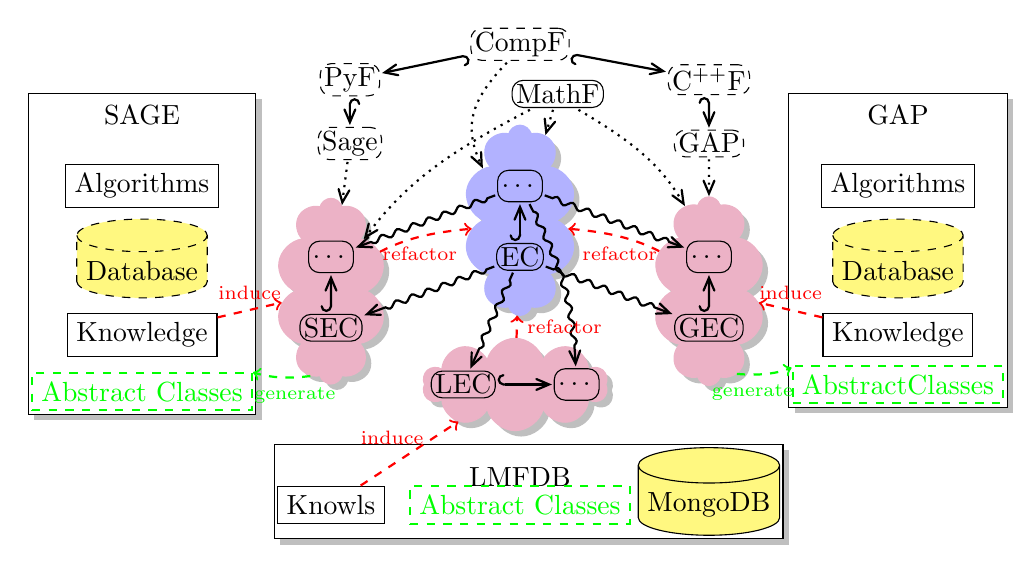
\begin{tikzpicture}[xscale=2.4,yscale=.9]
  \tikzstyle{withshadow}=[draw,drop shadow={opacity=.5},fill=white]
   \tikzstyle{database} = [cylinder,cylinder uses custom fill,
      cylinder body fill=yellow!50,cylinder end fill=yellow!50,
      shape border rotate=90,
      aspect=0.25,draw]
   \tikzstyle{human} = [red,dashed,thick]
   \tikzstyle{machine} = [green,dashed,thick]

\node[thy]  (mf) at (.2,5.3) {MathF};
\node[thy,dashed]  (compf) at (0,6) {CompF};
\node[thy,dashed]  (pf) at (-.9,5.5) {PyF};
\node[thy,dashed]  (cf) at (1,5.5) {C\textsuperscript{++}F};
\node[thy,dashed]  (sf) at (-0.9,4.6) {Sage};
\node[thy,dashed]  (gf) at (1,4.6) {GAP};

\draw[include] (compf) -- (pf);
\draw[includeleft] (compf) -- (cf);
\draw[include] (pf) -- (sf);
\draw[includeleft] (cf) -- (gf);

\node[thy] (kec) at (0,3) {EC};
\node[thy,minimum height=.4cm] (kl) at (0,4) {\ldots};

\node[thy] (sec) at (-1,2) {SEC};
\node[thy,minimum height=.4cm] (sl) at (-1,3) {\ldots};

\node[thy] (gec) at (1,2) {GEC};
\node[thy,minimum height=.4cm] (gl) at (1,3) {\ldots};

\node[thy] (lec) at (-.3,1.2) {LEC};
\node[thy,minimum height=.4cm] (ll) at (.3,1.2) {\ldots};

\node (sc) at (-2,5) {SAGE};
\node[draw] (salg) at (-2,4) {Algorithms};
\node[database,dashed] (sdb) at (-2,2.8) {Database};
\node[draw] (skr) at (-2,1.9) {Knowledge};
\node[draw,machine] (sac) at (-2,1.1) {Abstract Classes};

\node (gc) at (2,5) {GAP};
\node[draw] (galg) at (2,4) {Algorithms};
\node[database,dashed] (gdb) at (2,2.8) {Database};
\node[draw] (gkr) at (2,1.9) {Knowledge};
\node[draw,machine] (gac) at (2,1.2) {AbstractClasses};

\node (lmfdb) at (0,-.1) {LMFDB};
\node[database] (ldb) at (1,-.5) {MongoDB};
\node[draw] (knowls) at (-1,-.5) {Knowls};
\node[draw,machine] (lac) at (0,-.5) {Abstract Classes};

  \begin{pgfonlayer}{background}
    \node[draw,cloud,fit=(sec) (sl),aspect=.4,inner sep=-3pt,withshadow,purple!30] (st) {};
    \node[draw,cloud,fit=(gec) (gl),aspect=.4,inner sep=-4pt,withshadow,purple!30] (gt) {};
    \node[draw,cloud,fit=(kec) (kl),aspect=.4,inner sep=0pt,withshadow,blue!30] (kt) {};
    \node[draw,cloud,fit=(lec) (ll),aspect=3.5,inner sep=-8pt,withshadow,purple!30] (lt) {};
  \end{pgfonlayer}

\begin{pgfonlayer}{background}
  \node[draw,withshadow,fit=(sc) (skr) (sac) (sdb),inner sep=1pt] {};
  \node[draw,withshadow,fit=(gc) (gkr) (gac) (gdb),inner sep=1pt] {};
  \node[draw,withshadow,fit=(lmfdb) (lac) (ldb) (knowls),inner sep=1pt] {};
\end{pgfonlayer}

\draw[view] (kec) -- (sec);
\draw[view] (kec) -- (gec);
\draw[view] (kec) -- (lec);
\draw[include] (kec) -- (kl);
\draw[include] (gec) -- (gl);
\draw[include] (sec) -- (sl);
\draw[include] (lec) -- (ll);
\draw[view] (kl) -- (sl);
\draw[view] (kl) -- (gl);
\draw[view] (kl) to[bend left=5] (ll);

\draw[meta] (mf)  to [bend right=10] (st);
\draw[meta] (sf) -- (st);
\draw[meta] (mf)  to [bend left=10] (gt);
\draw[meta] (gf) -- (gt);
\draw[meta] (mf) -- (kt);
\draw[meta] (compf) to[bend right=15] (kt);

\draw[human,->] (skr) -- node[above]{\scriptsize induce} (st);
\draw[human,->] (gkr) -- node[above]{\scriptsize induce} (gt);
\draw[human,->] (knowls) -- node[left,near end]{\scriptsize induce} (lt);

\draw[machine,->] (gt) to[bend right=30] node[below,near start]{\scriptsize generate} (gac);
\draw[machine,->] (st) to[bend left=30] node[below,near start]{\scriptsize generate} (sac);
\draw[human,->] (st) to[bend left=20] node[below]{\scriptsize refactor} (kt);
\draw[human,->] (gt) to[bend right=20] node[below]{\scriptsize refactor} (kt);
\draw[human,->] (lt) -- node[right]{\scriptsize refactor} (kt);
\end{tikzpicture}
\end{document}
%%% Local Variables: 
%%% mode: latex
%%% TeX-master: t
%%% End: 

  \caption{The MitM paradigm in detail. PyF, C${}^{++}$F and CompF are (basic)
    foundational theories for \python, C${}^{++}$ and a generic computational model. SEC,
    LEC and GEC are theories for \SageMath, \LMFDB and \GAP elliptic curves.}\label{fig:mitm}
\end{figure}

A sketch of the theory graph based on the example of elliptic curves can be
found in Figure~\ref{fig:odk_theories}, an overview of the paradigm can be found
in Figure~\ref{fig:mitm}.  We will not go into details here but show how this
architecture integrates the \emph{Software} and \emph{Knowledge Aspects}.
Clearly, the MitM ontology -- the purple cloud in the middle -- is a
specification of the underlying mathematical knowledge as an OMDoc/MMT theory
graph, while the system interface theories -- the blue clouds around it --
formally specify the names and types (i.e. the argument patterns) and intended
behaviour of the interface functions of the systems (often semi-formally to make
the MitM approach scalable). The OMDoc/MMT views -- the wavy arrows between the
theories -- are interpretation morphisms; in this particular case where they
connect the mathematical specification to the system theories, they express the
``implementation relation''. Thus the OMDoc/MMT framework already allows to
integrate the knowledge and software aspects for system interoperability.

\subsection{Design Decisions and Initial Evaluation}
The MitM paradigm we choose for the software (S) aspect of the \pn VRE toolkit essentially
takes two design decisions:
\begin{compactenum}[\bf D1.]
\item The restriction to formalizing the interface specification (\textbf{S2.}: names and
  types of the interface functions) of the systems is sufficient to ensure system
  interoperability
\item integrating the implementations -- e.g. C\textsuperscript{++} or Python code -- into
  the OMDoc/MMT theories would be overkill here, since the code can only be executed by
  the respective systems -- i.e. \GAP or \SageMath. Therefore we will base our foundation
  on OMDoc/MMT theory graphs directly rather than on an extension of OMDoc/MMT with
  ``biform theories''~\cite{KohManRab:aumftg13,Farmer:btc07} as envisioned in the
  proposal. Biform theories would enable (partial) verification of mathematical software
  systems, but this is not on the critical path towards a mathematical VRE.
\end{compactenum}
The MitM paradigm constitutes a lightweight alternative; identifying and refining it has
been one of the major achievements of the first year in \WPref{dksbases}.

To evaluate the paradigm and the design decisions we have implemented extensions to the
\GAP and \SageMath that export interface theory graphs in the OMDoc/MMT format
(see~Section~\ref{sec:cases} for details):
\begin{compactitem}
\item \GAP exports types, constructors, functions, data, and their documentation: 4097
  Objects exported (2996 unique) in ca. 210 theories.
\item \SageMath exports categories/types, annotates functions: 382 Categories using 25
  Axioms and (in total) 808 methods.
\end{compactitem}
These interface theories allow the representation of all mathematical objects in \GAP and
\SageMath as OpenMath2/MathML3 objects~\cite{BusCapCar:2oms03,CarlisleEd:MathML3} whose
symbols are grounded in the interface theories (interpreted as OpenMath content
dictionaries). \GAP already had an \textbf{OpenMath phrasebook} -- an import/export
facility for OpenMath objects -- and we have developed one for Python and
\SageMath~\cite{py-openmath:on}.

Even though the development of the MitM paradigm is still at an early stage, these case
studies show the potential of the approach. We hope that the nontrivial cost of curating
an ontology of mathematical knowledge and interface views to the interface theories will
be offset by its utility as a resource, which we are currently exploring; the unification
of the knowledge representation components in the \MMT system
\begin{compactenum}
\item enables VRE-wide domain-centered (rather than system-centered) documentation: the
  namespace alignment given by the interface-views allows to re-use documentation for a
  concept, object, or model in the MitM ontology in all interface functions aligned with
  it.
\item can be leveraged for distributed computation via uniform protocols like the
  SCSCP~\cite{HorRoz:ossp09} and MONET-style service
  matching~\cite{CaprottiEtAl:MathServiceMatching04:tr} (the absence of content
  dictionaries -- now given as interface theories -- was the main hurdle that kept these
  from gaining more traction). Again, \GAP already had an SCSCP interface, and we are
  developing one for \SageMath at \cite{py-scscp:on}.
\item will lead to the wider adoption of best practices in mathematical knowledge
  management in the systems involved; in fact, this is already happening: the development
  of the \GAP interface theory exporter led to the discovery of hundreds of documentation
  errors and to a large-scale code refactoring that made type information more explicit
  and could lead to efficiency gains by extended static analysis in the future.
\end{compactenum}

%%% Local Variables:
%%% mode: latex
%%% TeX-master: "report"
%%% End:

%  LocalWords:  pn optimized behavior analyze compactenum textbf organization utilized
%  LocalWords:  characterized forall sqrt Leftrightarrow DehKohKon iop16 mitm centering
%  LocalWords:  myxscale myyscale emph emph formalizing KohManRab aumftg13 btc07 WPref
%  LocalWords:  dksbases compactitem domain-centered ossp09 py-scscp

\section{LMFDB knowledge and interoperability}\label{sec:lmfdb}
%\subsection{Short description of LMFDB's goals and implementation}
The \emph{$L$-functions and modular forms database} is a project involving dozens of
mathematicians who assemble computational data about $L$-functions, modular forms, and
related number theoretic objects. The main output of the project is a website, hosted at
\url{http://www.lmfdb.org}, that presents this data so that it can serve as a
reference for research efforts, and is accessible for postgraduate students.
The mathematical concepts underlying the \LMFDB are extremely complex and varied, so part
of the effort has been focused on how to relay knowledge, such as mathematical definitions
and their relationships, to data and software. For this purpose, the \LMFDB has developed so-called
\emph{knowls}, which are a technical solution to present \LaTeX-encoded information
interactively, heavily exploiting the concept of transclusion. The end result is a
very modular and highly interlinked set of definitions in mathematical vernacular
which can be easily anchored in vastly different contexts, such as an interface to a database,
to browsable data, or as constituents of an encyclopedia \cite{lmfdb-definitions}.

The \LMFDB code is primarily written in \Python, with some reliance on \Sage for
the business logic. The backend
uses the NoSQL document database system \Mongo \cite{lmfdb-repo}. Again, due to the
complexity of the objects considered, many idiosyncratic encodings are used for the
data. This makes the whole data management lifecycle particularly tricky, and dependent on
different select groups of individuals for each component.

%\subsection{Tentative approach to MMT semantic layers for the LMFDB}
As the LMFDB spans the whole ``vertical'' workflow, from writing software, to producing new
data, up to presenting this new knowledge, it is a perfect test case for a large scale
case study of the MitM approach. Conversely, a semantic layer would be beneficial to its
activities across data, knowledge and software, which it would help integrate more
cohesively and systematically.

Among the components of the LMFDB, elliptic curves stand
out in the best shape, and a source of best practices for other areas. 
%
% For this reason,
% the \ODK collaboration targeted that relatively small subset of the LMFDB for its
% prototype. We plan to extend coverage in a second phase, and expect it to be relatively
% easy if we manage to demonstrate the added value of a semantic layer for our prototype.
%
We have generated MitM interface theories for LMFDB elliptic curves by (manually)
refactoring and flexiformalizing the {\LaTeX} source of knowls into \sTeX (see
Listing~\ref{stex-ec} for an excerpt), which can be converted into flexiformal OMDoc/MMT
automatically. The MMT system can already type-check the definitions, avoiding circularity
and ensuring some level of consistency in their scope and make it browsable through
\textsf{MathHub.info}, a project developed in parallel to MMT to host such formalisations.

\lstinputlisting[language={[sTeX]TeX},label={stex-ec},firstline=31,
   caption= {\protect\stex flexiformalization of an \LMFDB knowl (original: \cite{lmfdb-mwm})}]
   {examples/elliptic-curve.tex}

   The second step consisted of translating these informal definitions into progressively
   more exhaustive MMT formalisations of mathematical concepts (see
   Listing~\ref{lst:mmt-ec}). The two representations are coordinated via the theory and
   symbol names -- we can see the \sTeX representation as a human-oriented documentation
   of the MMT.

\lstinputlisting[morekeywords={namespace,theory,include},mathescape,
firstline=21,
caption= {MMT formalisation of elliptic curves and their Weierstrass models},
label=lst:mmt-ec]{examples/elliptic-curve.mmt}


Finally, we have to integrate computational data into the interface theories. Based on
recent ongoing efforts \cite{lmfdb-formats} to document the \LMFDB ``data schemata'' we
established OMDoc/MMT theories that link the database fields to their data types (string
\emph{vs.} float \emph{vs.} integer tuple, for instance) and mathematical types (elliptic
curves or polynomials) -- the latter based on the vocabulary in the interface theories
generated from the \LMFDB knowls. This schema theory is complemented by a theory on
functorial hence composable \emph{MMT codecs}, which in turn acts as a specification for a collection of
implementations in various programming languages (currently \Python, Scala, and
C\textsuperscript{++} for \Sage, MMT, and \GAP respectively) which are first instances of
a computational foundation (see Section~\ref{sec:mitm}).  For instance, one can compose
two MMT codecs, say \emph{polynomial-as-reversed-list} and
\emph{rational-as-tuple-of-int}, to signify that the data $[(2,3),(0,1),(4,1)]$ is meant
to represent the polynomial $4x^2+2/3$. Of course, these codecs could be further
decomposed (e.g. for signaling which variable name to use). The initial cost of
developing these codecs is high, but the clarity gained in documentation is valuable, they
are highly reusable, and they drastically expand the range of tooling that can be built
around data management.


\paragraph{A typical application}
Based on these MitM interface theories we can generate I/O interfaces that translate
between the low-level \LMFDB API, which delivers raw \Mongo data in JSON format into MMT
expressions that are grounded in the interface theories. This ties the \LMFDB database
into the MitM architecture transparently. As a side effect, this opens up the \LMFDB to
programmatic queries via the MMT API, which can be queried and can then relay them to the
\LMFDB API directly and transparently.

%  LocalWords:  subsubsection emph knowls textsf lmfdb-repo stex-ec stex knowl mmt-ec odk
%  LocalWords:  Weierstrass emphasizing alltt tp rightarrow vdash doteq vdash doteq lst
%  LocalWords:  polynomial_equation_injectivity a_invariants_factors_injectivity colorbox
%  LocalWords:  minimality_idempotence lmfdb-formats emphasized composable standardize
%  LocalWords:  rda-typing lstinputlisting mathescape elliptic-curve.mmt lmfdb firstline

%%% Local Variables:
%%% mode: latex
%%% TeX-master: "paper"
%%% End:
%  LocalWords:  flexiformal flexiformalization flexiformalizing ednote mathhub mitm
%  LocalWords:  lmfdb-mwm functorial signaling

\section{Distributed collaboration with GAP/Sage}\label{sec:gapsage}
\label{sec:handles}

Another aspect of interoperability in a mathematical VRE is the possibility
of distributed multisystem computations, where \emph{e.g.}\ a given system
may decide to delegate certain subcomputations or reasoning tasks to other systems.

There are already a variety of peer-to-peer interfaces between systems
in the \ODK project (see Figure~\ref{fig:interop}), which are based on
the \emph{handle paradigm}; for example \Sage includes, among others,
interfaces for \GAP, \Singular, and \Pari.
%
In this paradigm, when a system $A$ delegates a calculation to a system $B$, the
result $r$ of the calculation is not converted to a native $A$ object; instead $B$ just
returns a \emph{handle} $h$ (or reference) to the object $r$. Later, $A$ can run further
calculations with $r$ by passing it as argument to functions or methods implemented by $B$.
Some advantages of this approach are that we can avoid the overhead of back and forth
conversions between $A$ and $B$, and that we can manipulate objects of $B$ from $A$, even
if they have no native representation in $A$.

The next desirable feature is for the handle $h$ to behave in $A$ as
if it was a native $A$ object; in other words, one wants to adapt the API
satisfied by $r$ in $B$ to match the API for the same kind of objects
in $A$. For example, the method call \texttt{h.cardinality()} on a
\Sage handle \texttt{h} to a \GAP object \texttt{G} should trigger in
\GAP the corresponding function call \texttt{Size(G)}.

This can be implemented using the classical \emph{adapter
  pattern}, mapping calls to \Sage's method to corresponding \GAP
methods. \emph{Adapter classes} have already been implemented for
certain types of objects, like \Sage's \texttt{PermutationGroup} or
\texttt{MatrixGroup}. However, this implementation lacks modularity:
for example, if \texttt{h} is a handle to a mere set \texttt{S}, \Sage
cannot use the \emph{adapter method} that maps
\texttt{h.cardinality()} to \texttt{Size(S)}, because this adapter
method is only available in the above two adapter classes.

To get around this problem we have worked on a more semantic
integration, where adapter methods are made aware of the type
hierarchies of the respective systems, and defined at the highest
available level of generality, as in Listing~\ref{lst:adapter}.
\begin{lstlisting}[language=Python,label=lst:adapter,
  caption=A semantic adapter method in \Sage]
class Sets: # Everything generic about sets in Sage
    class GAP: # Adapter methods relevant to Sets in the Sage-Gap interface
         class ParentMethods: # Adapter methods for sets
             def cardinality(self): # The adapter for the cardinality method
                 return self.gap().Size().sage()
         class ElementMethods: # Adapter methods for set elements
             ...
         class MorphismMethods: # Adapter methods for set morphisms
             ...
class Groups: # Everything generic about groups in Sage
     # This automatically includes features defined at a more general level
\end{lstlisting}

This peer-to-peer approach however does not scale up to a dozen
systems. This is where the MitM paradigm comes to the rescue. With it,
the task is reduced to building interface theories and interface views
into the core MitM ontology in such a way that the adapter pattern can be
made generic in terms of the MitM ontology structure, without relying
on the concrete structure of the respective type systems. Then the
adapter methods for each peer-to-peer interface can be automatically
generated.
%
In our example the adapter method for \texttt{cardinality} can be
constructed automatically as soon as the MitM interface views link the
\texttt{cardinality} function in the \Sage interface theory on Sets
with the \texttt{Size} function in the corresponding interface theory
for \GAP.

We will now show first results of our experiments with interface
theories and interface views, including several applications beyond the
generation of interface theories that support distributed computation
for \Sage and \GAP.

\subsection{Semantics in the \Sage category system}

The \Sage library includes 40k functions and allows for manipulating
thousands of different kinds of objects. In any large system it is
critical to tame code bloat by
\begin{compactenum}[\em i\rm)]
\item identifying the core concepts describing common behavior among the objects;
\item implementing generic operations that apply on all objects having a given
  behavior, with appropriate specializations when performance calls for it;
\item designing or choosing a process for selecting the best implementation available when
  calling an operation on some objects.
\end{compactenum}

Following mathematical tradition and the precedent of the \Axiom,
\Fricas, or \MuPAD systems, \Sage has developed a
category-theory-inspired ``category system'', and found a way to
implement it on top of the underlying \Python object
system~\cite{Sage,Sage.Categories}. In short, a \defemph{category} specifies
the available \defemph{operations} and the \defemph{axioms} they satisfy.
%
This category system models taxonomic knowledge from mathematics
explicitly and uses it to support genericity, control the method
selection process, structure the code and documentation, enforce
consistency, and provide generic tests.

% \ednote{NT: switch this example to (magmas, *)?}
% \ednote{NT: it would be nice to include here the MMT formalization of
%   Size/cardinality}
\begin{wrapfigure}r{8cm}\vspace*{-2.5em}
\begin{lstlisting}[language=Python,escapechar=!]
!\color{red}{@semantic(mmt="sets")}!
class Sets:
    class ParentMethods:
         !\color{red}{@semantic(mmt="card?card", gap="Size")}!
         @abstractmethod
         def cardinality(self):
             "Return the cardinality of ``self``"
\end{lstlisting}
\vspace*{-.5em}
\caption{An annotated category in \Sage}\label{fig:anncat}\vspace*{-1.5em}
\end{wrapfigure}
To generate interface theories from the \Sage category system, we are experimenting with a
system of annotations in the \Sage source files. Consider for instance the situtation in
Figure~\ref{fig:anncat} where we have annotated the \texttt{Sets()} category in \Sage
with \texttt{@semantic} lines that state correspondences to other interface theories. From
these the \Sage-to-MMT exporter can generate the respective interface theories and views.

In ongoing experiments, variants of the annotations are tested for
annotating existing categories without touching their source files and
providing the signature or the corresponding method names in other
systems when this information has not yet been formalized elsewhere.
% \ednote{POD: Would it be interesting to add a line about the constraints that are taken into consideration? For instance, the versioning of systems in parallel might become more problematic if it becomes so heavily interdependent}


\subsection{Exporting the \GAP knowledge: type system documentation}
\label{sec:gaptypes}

As in \Sage, the \GAP type system encodes a wealth of mathematical
knowledge, which can influence method selection. For example
establishing that a group is nilpotent will allow for more efficient
methods to be run for finding its centre. The main difference between \Sage
and \GAP lies in the method selection process. In \Sage the operations
implemented for an object and the axioms they satisfy are specified by
its class which, together with its super classes, groups syntactically
all the methods applicable in this context. In \GAP, this information
is instead specified by the truth-values of a collection of
independent \defemph{filters}, while the context of applicability is
specified independently for each method.
%
Breuer and Linton describe the \GAP type system in \cite{breuer-linton} and
the \GAP documentation \cite{GAP4} also contains extensive information on the types
themselves.

\begin{wrapfigure}r{6cm}%\vspace*{-2em}
  \includegraphics[width=6cm]{gap-graph.pdf}\vspace*{-.5em}
  \caption{The \GAP Knowledge Graph.\label{fig:gap-graph}}\vspace*{-2em}
\end{wrapfigure}
\GAP allows some introspection of this knowledge after the system is
loaded: the values of those attributes and properties that are unknown on creation,
can be computed on demand, and stored for later reuse.% without the need to be recomputed.

As a first step in generating interface theories for the MitM ontology, we have developed
tools to access mathematical knowledge encoded in \GAP, such as introspection inside a
running \GAP session, export to JSON to import to MMT, and export as a graph for
visualisation and exploration. These will become generally available in the next \GAP
release. The JSON output of the \GAP object system with default packages is currently
around 11 Megabytes, and represents a knowledge graph with 540 vertices, 759 edges
and 8 connected components, (see Figures~\ref{fig:gap-graph},\ref{fig:gap-ismagma}). If all
packages are loaded, this graph expands to 1616 vertices, 2178 edges and 17 connected
components.

There is, however, another source of knowledge in the \GAP universe: the documentation,
which is provided in the GAPDoc format \cite{gapdoc}. Besides the main manuals, GAPDoc
is adopted by 97 out of the 130 packages currently redistributed with
GAP. Conventionally GAPDoc is used to build text, PDF and HTML versions of the manual
from a common source given in XML. The reference manual has almost 1400 pages and the
packages add hundreds more.

The GAPDoc sources classify documentation by the type of the documented object (function,
operation, attribute, property, etc.) and index them by system name. In this sense they
are synchronized with the type system (which \emph{e.g.}\ has the types of the functions) and can
be combined into flexiformal OMDoc/MMT interface theories, just like the ones for \LMFDB
in Section~\ref{sec:lmfdb}. This conversion is currently under development and will lead
to a significant increase of the scope of the MitM ontology. 

\begin{figure}[ht]\centering
  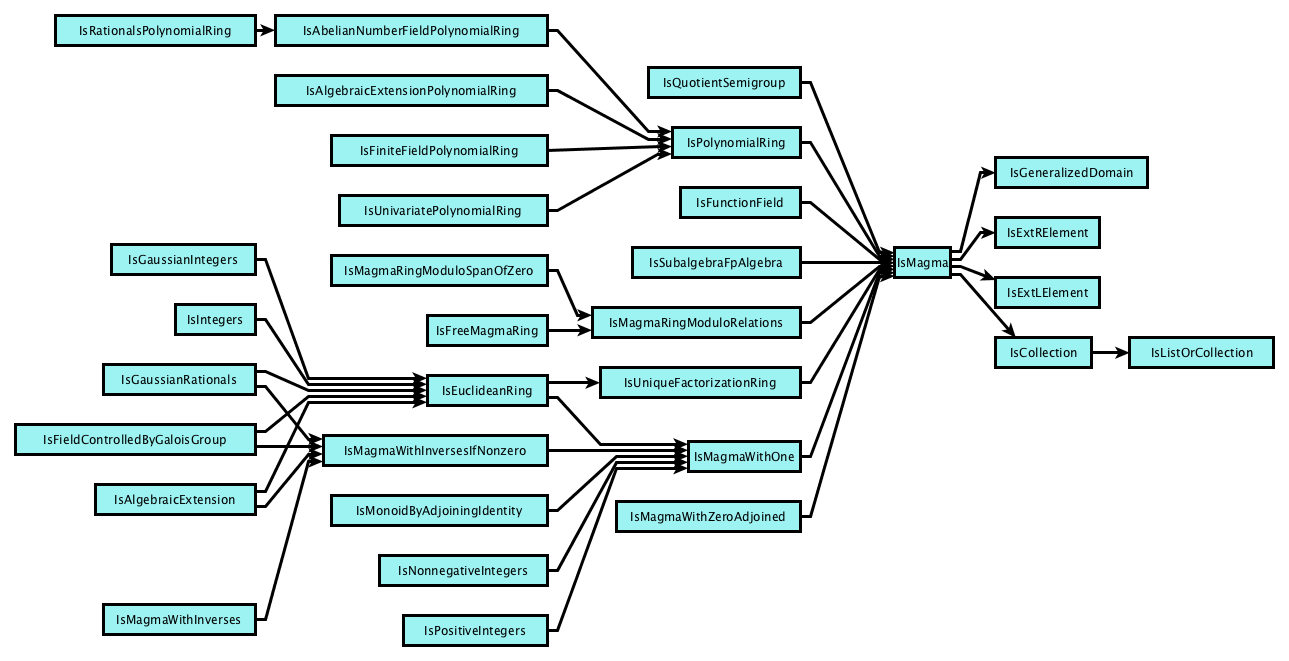
\includegraphics[width=\textwidth]{gap-ismagma}
  \caption{The \GAP Knowledge Graph (fragment).\label{fig:gap-ismagma}}
\end{figure}

As a side-effect of this work, we discovered quite a few inconsistencies in the \GAP
documentation which came from a semi-automated conversion of GAP manuals from the
\TeX-based manuals used in GAP 4.4.12 and earlier.  We developed the consistency checker
for the GAP documentation, which extracts type annotations from the documented GAP objects
and compares them with their actual types. It immediately reported almost 400
inconsistencies out of 3674 manual entries, 75\% of which have been
eliminated in the subsequent cleanup.

%%% Local Variables:
%%% mode: latex
%%% TeX-master: "paper"
%%% End:

%  LocalWords:  gapsage newpart texttt interop lst lstlisting Mehthod inparaenum behavior
%  LocalWords:  specializations ednote wrapfigure vspace mmt anncat formalized emph emph
%  LocalWords:  breuer-linton centering includegraphics gapdoc synchronized flexiformal
%  LocalWords:  lmfdb compactenum defemph formalization escapechar gaptypes textwidth

\section{Conclusion}\label{sec:concl}

We have shown how to extend the Math-in-the-Middle framework for integrating systems to mathematical data bases like the \lmfdb. 
The main idea is to embed knowledge sources as virtual theories, i.e. theories that are not -- theoretically or in practice -- limited in the number of declarations and allow dynamic loading and processing. 
For accessing real-world knowledge sources, we have developed the notion of codecs and integrated them into the MitM ontology framework. 
These codec's (and their MitM types) lift knowledge source access to the MitM level and thus enable object-level interoperability and allow humans (mathematicians) access using the concepts they are familiar with. 
Finally, we have shown a prototypical query translation facility that allows to delegate some of the processing to the underlying knowledge source and thus avoid thrashing of virtual theories. 

\paragraph{Related Work} Most other integration schemes employ a \textbf{homogenous approach}, where there is a master sytsem and all data is converted into that system. 
A paradigmatic example of this is the Wolfram Language and the Wolfram Alpha search engine~\cite{WolframAlpha:on}, which are based on the Mathematica kernel. 
This is very flexible for anyone owning a Matheamtica license and experienced in the Mathematica language and environment.

The MitM-based approach to interoperability of data sources and systems proposed in this paper is inherently a \textbf{heterogeneous approach}: systems and data sources are kept ``as is'', but their APIs are documented in a machine-actionable way that can be utilized for remote procedure calls, content format mediation, and service discovery. 
As a consequence, interaction between systems is very flexible.
For the data source integration via virtual theories presented in this paper this is important. 
For instance, we can just make an extension of \mmt or Sage which just act as a programmatic interface for e.g. \lmfdb. 

\paragraph{Future Work}
We have discussed the MitM+virtual theories methodology on the elliptic curves sub-base of the \lmfdb, which we have fully integrated. 
We are currently working on additional \lmfdb sub-bases. 
The main problem to be solved is to elicit the information for the respective schema theories from the \lmfdb community. 
Once that is accomplished, specifying them in the format discussed in this paper and writing the respective codecs is straightforward. 

Moreover, we are working on integrating the the Online Encyclopedia of Integer Sequences (OEIS~\cite{Sloane:OEIS,oeis}). 
Here we have a different problem: the OEIS database is essentially a flat ASCII file with different slots (for initial segments of the sequences, references, comments, and formulae); all minimally marked up ASCII art. 
In~\cite{LuzKoh:fsarfo16} we have already (heuristically) flexiformalized OEIS contents in \ommt; the next step will be to come up with codecs based on this basis and develop schema theories for OEIS.

\subsubsection*{Acknowledgements}
The authors gratefully acknowledge the fruitful discussions with other participants of
work package WP6, in particular John Cremona on the LMFDB and Dennis M\"uller on early
versions of the \ommt-based integration. We acknowledge financial support from the
OpenDreamKit Horizon 2020 European Research Infrastructures project (\#676541).

%%% Local Variables:
%%% mode: latex
%%% TeX-master: "paper"
%%% End:

%  LocalWords:  sec:concl subsubsection ommt lmfdb itemize Sloane:OEIS,oeis LuzKoh:fsarfo16 flexiformalized MitM-based textbf utilized


\printbibliography
\end{document}
%%% Local Variables:
%%% mode: latex
%%% TeX-master: t
%%% End:

%  LocalWords:  maketitle endeavor ednote ODKproposal printbibliography subsubsection pn
%  LocalWords:  IPython Jupyter emph itemize specialized Arxiv oldpart organization ec
%  LocalWords:  citability github Swinnerton-Dyer resentation desingularisation Hironaka
%  LocalWords:  Hironaka algorithmisation Villamayor visualization lstinline omtext lec
%  LocalWords:  multisystem-semantic-handle-interfaces.tex presenting-lmfdb.tex Dehaye
%  LocalWords:  Mihnea Iancu Konovalov Leli evre Wiesing odk mitm presenting-lmfdb concl
%  LocalWords:  multisystem-semantic-handle-interfaces
